\chapter{Coulombic Interaction} % Main chapter title
\label{Chapter2} % Change X to a consecutive number; for referencing this chapter elsewhere, use \ref{ChapterX}
\lhead{Chapter 2. \emph{Coulombic Interaction and Ewald Summation}} 

In this chapter, we provide a basic framework of Coulombic interaction and Ewald summation in a periodic system. Consider a 3D periodic system, which encloses $n_p$ charges in a simulation box. The box is infinitely repeated in all dimensions. For simplicity, we assume an orthorhombic periodic cell and therefore the coordinates of the ions can be obtained by translating along the lattice vectors. For a charge neutral system ($\sum_i q_i=0$) with $n_p$ point charges, $q_1,q_2....,q_{n_{p}}$ placed at $\vec{r_1},\vec{r_2},...,\vec{r_{n_p}}$, the energy of interaction (denoted as `$U$') of the ions in this unit cell with all the other ions and among themselves arising from Coulomb forces is given by
\begin{flalign}
    (4\pi\epsilon_o)U &= \frac{1}{2}\sum_{\vec{M}= -\infty}^{\infty}{' \sum_{i=1}^{n_p}\sum_{j=1}^{n_p} \frac{q_iq_j}{|\vec{r_i}-\vec{r_j}+\vec{M}.\vec{L}|}}.\label{eq:coul}
\end{flalign}
where $\vec{M} \in \mathbb{Z}^3$ indexes all periodic images of the simulation box of sides $\vec L$, and the prime (${}^\prime$) symbol is introduced to exclude the term $j = i$ in the summation, when $\vec{M}=0 $. The summation is conditionally convergent, meaning that the final value depends on the specific order in which the terms are summed. Given that $\rho(\vec{r})$ is the charge density at any point $\vec{r}$ and $\phi(\vec{r})$ is the potential field at point $\vec{r}$, the summation can be rewritten as:
\begin{flalign}
     (4\pi\epsilon_o)U &= \frac{1}{2} \int_{-\infty}^{\infty} d\vec{r_2}\, \rho(\vec{r_2}) \int_{-\infty}^{\infty} \frac{d\vec{r_1}\, \rho(\vec{r_1})}{|\vec{r_1}-\vec{r_2}|} \\
     &= \frac{1}{2}\int_{-\infty}^{\infty} d\vec{r_2}\, \rho(\vec r_2)\phi(\vec r_2)
\end{flalign}
For a point charge system, $\rho(\vec{r})$ is given by
\begin{equation}
    \rho(\vec{r})=\sum_{\vec{M}=-\infty}^{\infty}\sum_{j=1}^{n_p}q_j\delta(\vec{r}-\vec{r_j}+\vec{M}.\vec{L})
\end{equation}
To simulate an ionic system, it is essential to compute these interactions acting on each ion. However, the computational cost of these calculations typically scales quadratically with the number of ions, i.e., $O(N^2)$. This becomes computationally prohibitive for realistic molecular simulations involving as many as $10^5$ ions with \ac{PBC}.

\section{Ewald Summation Method}
The Ewald summation method, developed by Ewald~\cite{Ewald1921}, is a classical approach used to compute long-range Coulombic interactions in periodic systems. Ewald proposed decomposing the $1/r$ potential into two rapidly converging parts
\begin{flalign*}
\frac{1}{r} = \frac{{erfc}(\alpha r)}{r} + \frac{{erf}(\alpha r)}{r}
\end{flalign*}
Here, $\alpha$ is the Ewald splitting parameter that controls the convergence of the two parts. The first term represents a short-range interaction energy ($U^{SR}$) computed in real space, while the second term corresponds to a long-range interaction energy ($U^{LR}$) evaluated in reciprocal (Fourier) space. Additionally, a self-interaction energy ($U^{S}$) is added to the long-range term to make periodic and later subtracted.

$\therefore$ The total electrostatic energy is computed by evaluating three terms: 
\begin{flalign}
U = U^{SR} + U^{LR} + U^{S}.
\end{flalign}
This decomposition ensures convergence, and the computational cost can be significantly reduced by applying techniques amenable to such sums. 

% \swb{You have not defined the notations, e.g., $U^{LR}$.}

\subsection{Three-Dimensional Periodic Systems}
We begin by defining a reciprocal lattice vector $\vec{G}$ as $\vec G =  \frac{k_x2\pi}{L_x}\hat x+\frac{k_y2\pi}{L_y}\hat y+\frac{k_z2\pi}{L_z}\hat z$ 
% @@@Prateek: definition of k is not clear@@@
,where $k_x$, $k_y$, $k_z$ $\in$ $\mathbb{Z}$, and the structure factor $S(\vec G)$ as
\begin{flalign}
    S(\vec G) &= \sum_{j=1}^{n_p}q_j\,exp(i\vec G.\vec r_j).
\end{flalign}
Coulombic interaction given by Eq.~(\ref{eq:coul}) for a three-dimensional periodic system is expressed using the Ewald summation as
\begin{flalign}
    \nonumber (4\pi\epsilon_o)U &= U^{LR} + U^{S} + U^{SR}
\end{flalign}
Each of these terms is written as
\begin{flalign}
    U^{LR}& =\frac{2\pi}{L_xL_yL_z}\sum_{\mathbf{k}=-\infty}^{\infty}{}^{\prime}\frac{1}{|\vec{G}|^2}\,{exp}\left(\frac{-1}{4\alpha^2}|\vec{G}|^2\right)|\,S(\vec{G})\,|^2\, \\
    U^{S} &= -\frac{\alpha}{\sqrt{\pi}}\sum_{i=1}^{n_p} q_i^2  \\
    U^{SR}&=\frac{1}{2}\sum_{i=1}^{n_p}{}^\prime\sum_{j=1}^{n_p}q_i q_j\frac{erfc(\alpha|\vec{r_j}-\vec{r_i}|)}{|\vec{r_j}-\vec{r_i}|}
\end{flalign}
The computational cost of the traditional Ewald summation method, which scales as $O(N^2)$ and can be reduced to $O(N^\frac{3}{2})$ with optimised approaches, remains prohibitive for extensive molecular simulations\cite{frenkel2002understanding}. This limitation has motivated the development of more efficient techniques such as the Particle Mesh Ewald (PME)\cite{hockney2021computer} and \aclu{SPME} (\ac{SPME})\cite{SPME} methods.

The electrostatic force on $i^{th}$ atom in each direction ($\beta = x,y,z$) can be obtained by taking a derivative of the above components with respect to $\vec{r_{\beta i}}$. Each of the individual term would be defined as $\partial U^{LR}/\partial  r_{\beta i}$ (reciprocal space force), $\partial U^{SR}/\partial r_{\beta i}$ (real space force) and $\partial U^{S}/\partial r_{\beta i}$ (correction force).

\subsection{Smooth Particle Mesh Ewald}
The particle mesh Ewald method was first introduced by Hockney and Eastwood~\cite{hockney2021computer} utilising Laplace interpolation techniques to assign charges onto a regular grid. However, the discontinuous nature of Laplace interpolations posed challenges in accurately computing forces. To address this, the \ac{SPME} method was later developed by Essmann \textit{et al.}~\cite{SPME} which employs exponential B-splines to smoothly interpolate the charge distribution on the grid, enabling more accurate and efficient computations. These approaches employ fast fourier transform (FFT), thereby decreasing the computational complexity from $O(N^2)$ to $O[Nlog(N)]$, with a multiplicative constant that varies based on the desired level of accuracy.

In the \ac{SPME} method, the structure factor in the reciprocal space sum is expressed as
\begin{equation}
\exp(2\pi i \mathbf{k} \cdot \mathbf{r}) =
\exp\left(2\pi i \frac{k_x u_1}{K_1} \right)
\exp\left(2\pi i \frac{k_y u_2}{K_2} \right)
\exp\left(2\pi i \frac{k_z u_3}{K_3} \right),
\end{equation}
where $\mathbf{u} = \mathbf{K}.\mathbf{r}$ are the scaled fractional coordinates, where $\mathbf{K}$ is the grid points vector. To efficiently compute this on a mesh, each term is approximated using exponential B-splines
\begin{equation}
    \exp\left(2\pi i \frac{k_\lambda}{K_\lambda} u_\lambda\right) \approx 
    b \left(2\pi \frac{k_\lambda}{K_\lambda},n\right) \sum_{m=-\infty}^{\infty} M_n(u_\lambda - m) 
    \cdot \exp\left(2\pi i \frac{k_\lambda}{K_\lambda} m\right),\label{eq:bspline}
\end{equation}
and $\lambda$ is the direction ($\lambda = $ x, y, z) and $n$ as the order of B-spline interpolation, with normalisation
\begin{equation}
    b(u,v) = \frac{\exp\left(i (v - 1) u\right)}
       {\sum_{m=0}^{n-2} M_n(m+1) \exp\left(i um\right)}
\end{equation}
The B-spline functions are defined recursively. The second-order B-spline is 
$M_2(u) = 
1 - |u - 1| \text{ for } 0 \le u \le 2$, and zero otherwise, and for higher orders \( n > 2 \), the recursion is defined by Cox-de Boor formula~\cite{de1968uniform, de1972calculating} as 
\begin{equation}
M_n(u) = \frac{u}{n-1} M_{n-1}(u) + \frac{n - u}{n - 1} M_{n-1}(u - 1).
\end{equation}
The structure factor can be expressed as follows
\begin{equation}
    S(\vec{G}) \approx b\left(2\pi \frac{k_x}{K_x},n\right)\,b\left(2\pi \frac{k_y}{K_y},n\right)\,b\left(2\pi \frac{k_z}{K_z},n\right) \, \mathcal{F}_{3D}(Q)
\end{equation}
where $\mathcal{F}_{3D}(Q)$ is the 3D fourier transform of the array Q of interpolated charges on the grids with respect to $t_x,\,t_y\,$ and $t_z$, given by
\begin{equation}
    Q(t_x, t_y, t_z) =  \sum_{i=1}^{N} \sum_{n_1, n_2, n_3} q_i M_n(u_{1i} - t_x - n_1 K_1) \times M_n(u_{2i} - t_y - n_2 K_2) \times M_n(u_{3i} - t_z - n_3 K_3)
\end{equation}
With $ B_{3D}(k_x, k_y, k_z)$ defined as $$ B_{3D}(k_x, k_y, k_z) = \left| b\left(2\pi \frac{k_x}{K_x},n\right) \right|^2 \cdot \left| b\left(2\pi \frac{k_y}{K_y},n\right) \right|^2 \cdot \left| b\left(2\pi \frac{k_z}{K_z},n\right) \right|^2$$
Define $\chi(p_1,p_2,p_3)$ as
\begin{flalign}
    \nonumber \chi(p_x,p_y,p_z) &= \frac{2\pi}{L_xL_yL_z}\sum_{\vec{\mathbf{k}}=-\infty}^{\infty}{}^\prime \frac{1}{|\vec{G}|^2}\,{exp}\left(\frac{-1}{4\alpha^2}|\vec{G}|^2\right)\,\times B_{3D}(k_x,k_y,k_z)
    \\&\quad\quad\quad\times \exp\left( i \frac{2\pi k_x p_x}{K_x} + i \frac{2\pi k_y p_y}{K_y} + i \frac{2\pi k_z p_z}{K_z} \right)
    \\&=\mathcal{F}_{3D}(E_{3D}.B_{3D})(p_x,p_y,p_z)
\end{flalign}
where the screening factor array $E_{3D}$ is defined as
\begin{flalign}
    E_{3D}(k_x,k_y,k_z) &=\frac{2\pi}{L_xL_yL_z} \frac{1}{|\vec{G}|^2}\,{exp}\left(\frac{-1}{4\alpha^2}|\vec{G}|^2\right)
\end{flalign}
Note that $E_{3D}\cdot B_{3D} = \mathcal{F}^{-1}_{3D}(\chi)$. The approximate reciprocal space sum is thus given as
\begin{flalign}
    \nonumber(4\pi\epsilon_o)U^{LR}  & \approx \frac{2\pi}{L_xL_yL_z}\sum_{\mathbf{k}=-\infty}^{\infty}{}^{\prime}\frac{1}{|\vec{G}|^2}\,{exp}\left(\frac{-1}{4\alpha^2}|\vec{G}|^2\right)\, B_{3D}(k_x,k_y,k_z)  \\
    &\quad\quad\quad\quad\quad\cdot \left|\mathcal{F}_{3D}(Q)(k_x,k_y,k_z)\right|^2 \\ \label{eq:reci3DSPME}
    \nonumber &= \sum_{k_x=0}^{K_1-1} \sum_{k_y=0}^{K_2-1} \sum_{k_z=0}^{K_3-1}\mathcal{F}^{-1}_{3D}(\chi)(k_x,k_y,k_z)\cdot \mathcal{F}_{3D}(Q)(k_x,k_y,k_z) \\
    \nonumber &\quad\quad\quad\quad\quad\cdot K_xK_yK_z\,\mathcal{F}^{-1}_{3D}(Q)(k_x,k_y,k_z) \\
    &=\sum_{k_x=0}^{K_1-1} \sum_{k_y=0}^{K_2-1} \sum_{k_z=0}^{K_3-1} Q(k_x,k_y,k_z) \cdot (\chi \star Q)(k_x,k_y,k_z)
\end{flalign}
where $\star$ is the convolution operation expressed as
\begin{flalign}
    \chi \star Q(k_x,k_y,k_z) &= \sum_{k_x^\prime=0}^{K_1-1} \sum_{k_y^\prime=0}^{K_2-1} \sum_{k_z^\prime=0}^{K_3-1} \chi (k_x^\prime,k_y^\prime,k_z^\prime) \times Q (k_x-k_x^\prime,k_y-k_y^\prime,k_z-k_z^\prime)
\end{flalign}
As the array \(\chi\) is independent of the spatial orientation of the particles, the reciprocal space force  can therefore be expressed as follows
\begin{flalign}
    \frac{\partial U^{LR}}{\partial r_{\beta i}} &= 2\sum_{k_x=0}^{K_1-1} \sum_{k_y=0}^{K_2-1} \sum_{k_z=0}^{K_3-1} \frac{\partial Q(k_x,k_y,k_z)}{\partial r_{\beta i}} \cdot (\chi \star Q)(k_x,k_y,k_z)
\end{flalign}

\subsection{Slab-Type (Two-Dimensional Periodic) Systems}
In this section, we provide the basic framework for 2D periodic systems. We begin by defining $\sigma(k_{x}) = \frac{2\pi k_{x}}{L_{x}}$ and $\psi(k_{y}) = \frac{2\pi k_{y}}{L_{y}}$. Using these definitions, the structure factor is represented as
\begin{flalign}
    S(\vec{K},h) =\sum_{j=1}^{n_p}q_j\,exp[i(\sigma(k_x)x_{j} + \psi(k_y)y_{j}+hz_{j})] \label{eq:structurefactor}
\end{flalign}
The Coulombic interaction in Eq.~(\ref{eq:coul}) for a two-dimensional periodic system is expressed using the Ewald summation (2D-EW\cite{kawata2001rapid}) as
\begin{flalign}
    \nonumber (4\pi\epsilon_o)U &= U^{LR}_{k\neq0} +U^{LR}_{k=0} + U^{S} + U^{SR}.
\end{flalign}
Each of these terms is written as
\begin{flalign}
    U^{LR}_{k\neq0}  &= \frac{1}{L_xL_y} \sum_{\mathbf{k}=-\infty}^{\infty} {}^\prime 
    \int_{-\infty}^{\infty} dh\, \frac{\,{exp}\left(-\frac{\sigma^2+\psi^2 +h^2}{4\alpha^2}\right)}
    {\sigma^2+\psi^2 +h^2} \, |S(\vec{K},h)|^2,  \\
     U^{LR}_{k=0} &= \frac{2\sqrt{\pi}}{L_xL_y} \sum_{i=1}^{n_p}\sum_{j=1}^{n_p}q_i q_j
    \left[\frac{1-\,{exp}(-z_{ij}^2\alpha^2)}{\alpha}+\sqrt{\pi}z_{ij}\,{erf}(\alpha z_{ij})\right] \\
    U^S&= -\frac{\alpha}{\sqrt{\pi}}\sum_{i=1}^{n_p} q_i^2, \\
    U_{SR}&=\frac{1}{2}\sum_{i=1}^{n_p}{}^\prime\sum_{j=1}^{n_p} q_i q_j\frac{erfc(\alpha|\vec{r_j}-\vec{r_i}|)}{|\vec{r_j}-\vec{r_i}|}.
\end{flalign}
The derivation of these equations can be found in previous literature.@@@Prateek: cite the first paper on this@@@ For the reciprocal space summation, the absence of periodicity along the $z$-direction leads to an integral over this coordinate. Consequently, the summation over $k_z$, discrete in a fully periodic system, becomes a continuous Fourier transform. The real-space contribution to the Ewald summation remains the same in three-dimensional and two-dimensional periodic cases, with the only difference being the choice of the minimum image convention appropriate to each geometry. 

\subsection{2D-Particle Mesh Ewald (2D-PME)}
In the \aclu{2D-PME} (\ac{2D-PME}) \cite{kawata2001particle,kawata} method, the structure factor in the reciprocal space sum is expressed as 
\begin{equation}
\exp(2\pi i \mathbf{k} \cdot \mathbf{r'}) =
\exp\left(2\pi i \frac{k_x u_1}{K_1} \right)
\exp\left(2\pi i \frac{k_y u_2}{K_2} \right),
\end{equation}
where $\mathbf{r'}$ denotes the component of $\mathbf{r}$ confined to the (x, y) plane, and $\mathbf{u} = \mathbf{K}.\mathbf{(r')}$ represents the scaled fractional coordinates, with $\mathbf{K}$ being the vector corresponding to the grid points.
These exponential terms are evaluated using exponential B-splines, as defined in Eq. (\ref{eq:bspline}). Meanwhile, the $z$-direction term of the structure factor is approximated as
\begin{flalign}
    exp(ihz) \approx b(h,n)\times \sum_{t = -\infty}^{\infty} M_n[z - t]exp(iht)
\end{flalign}
The 2D structure factor from Eq. (\ref{eq:structurefactor}) can now be approximated as
\begin{flalign}
    \nonumber S(\vec{K},h) & \approx b\left(2\pi \frac{k_x}{K_x},n\right)\,b\left(2\pi \frac{k_y}{K_y},n\right)\, b(h,n) \,
    \\ & \sum_{t_x=0}^{K_x-1} \sum_{t_y=0}^{K_y-1} \sum_{t_z=-\infty}^{\infty}\left[ Q(t_x, t_y, t_z) \times \exp\left( i \frac{2\pi k_x t_x}{K_x} + i \frac{2\pi k_y t_y}{K_y} + i h t_z \right) \right]
\end{flalign}
The array Q of interpolated charges on the grids, given by
\begin{equation}
    Q(t_x, t_y, t_z) = \sum_{i=1}^{N} \sum_{n_1, n_2} q_i M_n(u_{1i} - t_x - n_1 K_1) \times M_n(u_{2i} - t_y - n_2 K_2) \times M_n(z_{i} - t_z)
\end{equation}
With $ B_{2D}(k_x, k_y, h)$ defined as $$ B_{2D}(k_x, k_y, h) = \left| b\left(2\pi \frac{k_x}{K_x},n\right) \right|^2 \cdot \left| b\left(2\pi \frac{k_y}{K_y},n\right) \right|^2 \cdot \left| b\left(h,n\right) \right|^2$$ 
The 2D-PME long-range interaction can be expressed as
\begin{flalign}
    (4\pi\epsilon_o)U^{LR} &\approx \frac{1}{L_xL_y} \sum_{k_x,k_y = -\infty}^{\infty}\int_{-\infty}^{\infty}dh\, B_{2D}(k_x,k_y,h)\frac{\,{exp}\left(-\frac{\sigma^2+\psi^2 +h^2}{4\alpha^2}\right)}{\sigma^2+\psi^2 +h^2} \, \left|\tilde{Q}(k_x,k_y,h)\right|^2
\end{flalign}
where $\tilde{Q}(k_x,k_y,h)$ is the 1D fourier integral of ${Q^\prime}(k_x,k_y,t_z)$ with respect to $t_z$ and ${Q^\prime}(k_x,k_y,t_z)$ is the 2D discrete fourier transform of $Q(t_x, t_y, t_z)$ with respect to $t_x$ and $t_y$. Define array $\theta(p_1,p_2,p_3)$ as
\begin{flalign}
    \nonumber \theta(p_x,p_y,p_z) &= \frac{1}{L_xL_y}\sum_{k_x,k_y = -\infty}^{\infty}{}^\prime \int_{-\infty}^{\infty}dh\, \frac{\,{exp}\left(-\frac{\sigma^2+\psi^2 +h^2}{4\alpha^2}\right)}{\sigma^2+\psi^2 +h^2} \,B_{2D}(k_x,k_y,h)
    \\&\quad\quad\quad\times \exp\left( i \frac{2\pi k_x p_x}{K_x} + i \frac{2\pi k_y p_y}{K_y} +  i h p_z \right)
    % \\&=\mathcal{F}_{3D}(E_{3D}.B_{3D})(p_x,p_y,p_z)
\end{flalign}
gives a simplified expression of the reciprocal space energy as
\begin{flalign}
     (4\pi\epsilon_o)U^{LR} &=\sum_{k_x=0}^{K_1-1} \sum_{k_y=0}^{K_2-1} \sum_{k_z=-\infty}^{\infty} Q(k_x,k_y,k_z) \cdot (\theta \star Q)(k_x,k_y,k_z)
\end{flalign}
where $\star$ is the convolution operation expressed as
\begin{flalign}
    \theta \star Q(k_x,k_y,k_z) &= \sum_{k_x^\prime=0}^{K_1-1} \sum_{k_y^\prime=0}^{K_2-1} \sum_{k_z^\prime=-\infty}^{\infty} \theta (k_x^\prime,k_y^\prime,k_z^\prime) \times Q (k_x-k_x^\prime,k_y-k_y^\prime,k_z-k_z^\prime)
\end{flalign}
The 2D-reciprocal space force can therefore be derived as
\begin{flalign}
      \frac{\partial U^{LR}}{\partial r_{\beta i}} &= 2\sum_{k_x=0}^{K_1-1} \sum_{k_y=0}^{K_2-1} \sum_{k_z^\prime=-\infty}^{\infty} \frac{\partial Q(k_x,k_y,k_z)}{\partial r_{\beta i}} \cdot (\theta \star Q)(k_x,k_y,k_z)
\end{flalign}

For the complete code implementations of this program refer to Appendix \ref{AppendixB}

\section{Need for Faster 2D Methods}
\begin{figure}[H]
    \centering
    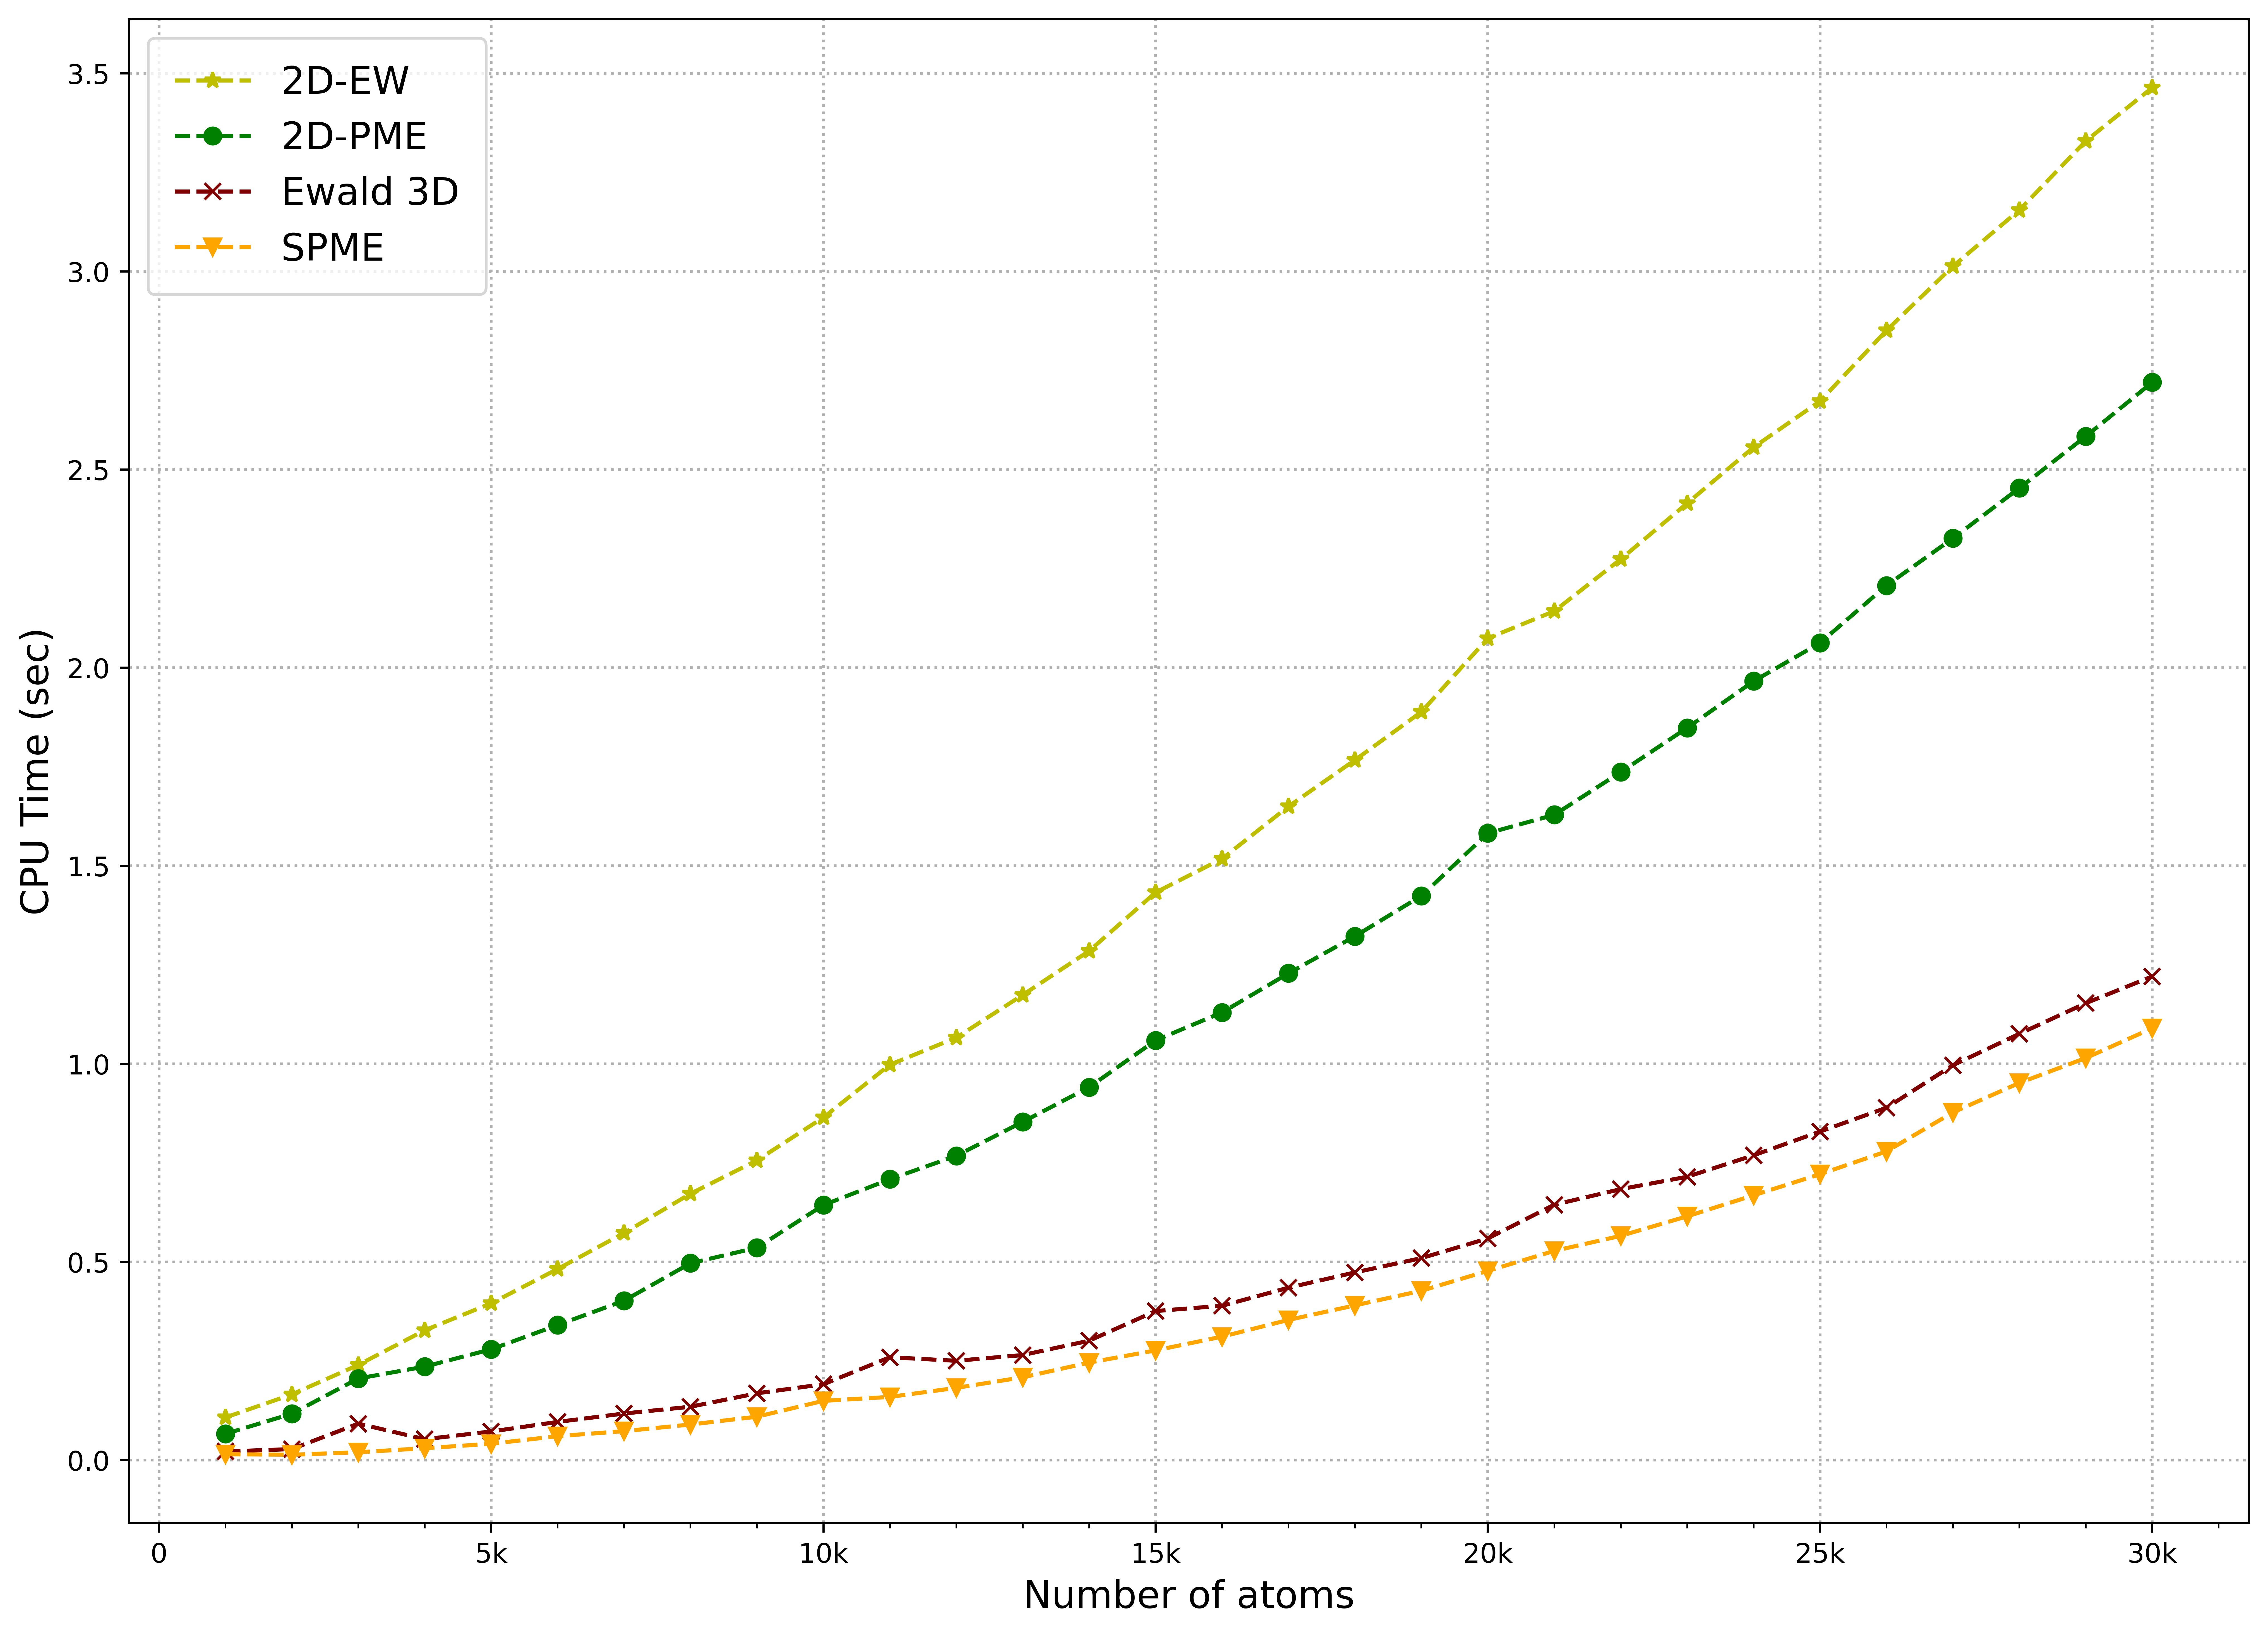
\includegraphics[width=1\linewidth]{images/kAWATA_VS_SPME_Result30k_3DEwald.jpg}
    \caption{Comparison of the CPU-times of the 3D and 2D Ewald methods with their particle mesh approach for the calculation of total Coulombic energies. Parameters for the particle mesh implementation were chosen to maintain high accuracy. For the \ac{SPME} method, a grid size of 64 and an interpolation order of 8 were used. For the 2D-PME method, grid sizes of 64 in the x and y directions and 128 in the z direction were taken, with an interpolation order of 8.}
    \label{fig:enter-label}
\end{figure}